%%%%%%%%%%%%%%%%%
% From Template %
%%%%%%%%%%%%%%%%%

\documentclass[%
class=scrreprt,
chapterprefix=false,%
open=right,%
twoside=false,%
paper=a4,%
logofile={Logo\_zentral\_farbig\_EN.png},%
thesistype=masterproposal,%
UKenglish,%
]{se2thesis}
\listfiles
\usepackage[ngerman,main=UKenglish]{babel}
\usepackage{blindtext}
\usepackage[%
csquotes=true,%
booktabs=true,%
siunitx=true,%
minted=true,%
selnolig=true,%
widowcontrol=false,%
microtype=true,%
% biblatex=true,%
cleveref=true,%
]{se2packages}

% Own change (from Lisa)
% Changing citeauthor to use et el.
\usepackage[maxcitenames=2,backend=biber]{biblatex}
% End own change

\begin{filecontents}{\jobname.bib}
	@article{boehm2001defect,
		title={Defect reduction top 10 list},
		author={Boehm, Barry and Basili, Victor R},
		journal={Computer},
		volume={34},
		number={1},
		pages={135--137},
		year={2001}
	}
	
	@article{buse2009learning,
		title={Learning a metric for code readability},
		author={Buse, Raymond PL and Weimer, Westley R},
		journal={IEEE Transactions on software engineering},
		volume={36},
		number={4},
		pages={546--558},
		year={2009},
		publisher={IEEE}
	}
	
	@inproceedings{aggarwal2002integrated,
		title={An integrated measure of software maintainability},
		author={Aggarwal, Krishan K and Singh, Yogesh and Chhabra, Jitender Kumar},
		booktitle={Annual Reliability and Maintainability Symposium. 2002 Proceedings (Cat. No. 02CH37318)},
		pages={235--241},
		year={2002},
		organization={IEEE}
	}
	
	@inproceedings{fakhoury2019improving,
		title={Improving source code readability: Theory and practice},
		author={Fakhoury, Sarah and Roy, Devjeet and Hassan, Adnan and Arnaoudova, Vernera},
		booktitle={2019 IEEE/ACM 27th International Conference on Program Comprehension (ICPC)},
		pages={2--12},
		year={2019},
		organization={IEEE}
	}
	
	@inproceedings{scalabrino2016improving,
		title={Improving code readability models with textual features},
		author={Scalabrino, Simone and Linares-Vasquez, Mario and Poshyvanyk, Denys and Oliveto, Rocco},
		booktitle={2016 IEEE 24th International Conference on Program Comprehension (ICPC)},
		pages={1--10},
		year={2016},
		organization={IEEE}
	}
	
	@inproceedings{posnett2011simpler,
		title={A simpler model of software readability},
		author={Posnett, Daryl and Hindle, Abram and Devanbu, Premkumar},
		booktitle={Proceedings of the 8th working conference on mining software repositories},
		pages={73--82},
		year={2011}
	}
	
	@article{dorn2012general,
		title={A general software readability model},
		author={Dorn, Jonathan},
		journal={MCS Thesis available from (http://www. cs. virginia. edu/weimer/students/dorn-mcs-paper. pdf)},
		volume={5},
		pages={11--14},
		year={2012}
	}
	
	@inproceedings{scalabrino2017automatically,
		title={Automatically assessing code understandability: How far are we?},
		author={Scalabrino, Simone and Bavota, Gabriele and Vendome, Christopher and Linares-V{\'a}squez, Mario and Poshyvanyk, Denys and Oliveto, Rocco},
		booktitle={2017 32nd IEEE/ACM International Conference on Automated Software Engineering (ASE)},
		pages={417--427},
		year={2017},
		organization={IEEE}
	}
	
	@inproceedings{daka2015modeling,
		title={Modeling readability to improve unit tests},
		author={Daka, Ermira and Campos, Jos{\'e} and Fraser, Gordon and Dorn, Jonathan and Weimer, Westley},
		booktitle={Proceedings of the 2015 10th Joint Meeting on Foundations of Software Engineering},
		pages={107--118},
		year={2015}
	}
	
	@article{mi2022towards,
		title={Towards using visual, semantic and structural features to improve code readability classification},
		author={Mi, Qing and Hao, Yiqun and Ou, Liwei and Ma, Wei},
		journal={Journal of Systems and Software},
		volume={193},
		pages={111454},
		year={2022},
		publisher={Elsevier}
	}
	
	@inproceedings{mi2018gamification,
		title={A gamification technique for motivating students to learn code readability in software engineering},
		author={Mi, Qing and Keung, Jacky and Mei, Xiupei and Xiao, Yan and Chan, WK},
		booktitle={2018 International Symposium on Educational Technology (ISET)},
		pages={250--254},
		year={2018},
		organization={IEEE}
	}
	
	@article{mi2018improving,
		title={Improving code readability classification using convolutional neural networks},
		author={Mi, Qing and Keung, Jacky and Xiao, Yan and Mensah, Solomon and Gao, Yujin},
		journal={Information and Software Technology},
		volume={104},
		pages={60--71},
		year={2018},
		publisher={Elsevier}
	}
	
	@book{brooks1987no,
		title={No silver bullet},
		author={Brooks, Frederick and Kugler, H},
		year={1987},
		publisher={April}
	}
	
	@article{loriot2022styler,
		title={Styler: learning formatting conventions to repair Checkstyle violations},
		author={Loriot, Benjamin and Madeiral, Fernanda and Monperrus, Martin},
		journal={Empirical Software Engineering},
		volume={27},
		number={6},
		pages={149},
		year={2022},
		publisher={Springer}
	}
	
	@inproceedings{yasunaga2020graph,
		title={Graph-based, self-supervised program repair from diagnostic feedback},
		author={Yasunaga, Michihiro and Liang, Percy},
		booktitle={International Conference on Machine Learning},
		pages={10799--10808},
		year={2020},
		organization={PMLR}
	}
	
	@inproceedings{xu2019method,
		title={Method name suggestion with hierarchical attention networks},
		author={Xu, Sihan and Zhang, Sen and Wang, Weijing and Cao, Xinya and Guo, Chenkai and Xu, Jing},
		booktitle={Proceedings of the 2019 ACM SIGPLAN workshop on partial evaluation and program manipulation},
		pages={10--21},
		year={2019}
	}
	
	@inproceedings{allamanis2016convolutional,
		title={A convolutional attention network for extreme summarization of source code},
		author={Allamanis, Miltiadis and Peng, Hao and Sutton, Charles},
		booktitle={International conference on machine learning},
		pages={2091--2100},
		year={2016},
		organization={PMLR}
	}
	
	@article{hestness2017deep,
		title={Deep learning scaling is predictable, empirically},
		author={Hestness, Joel and Narang, Sharan and Ardalani, Newsha and Diamos, Gregory and Jun, Heewoo and Kianinejad, Hassan and Patwary, Md Mostofa Ali and Yang, Yang and Zhou, Yanqi},
		journal={arXiv preprint arXiv:1712.00409},
		year={2017}
	}
	
	@inproceedings{liu2019learning,
		title={Learning to spot and refactor inconsistent method names},
		author={Liu, Kui and Kim, Dongsun and Bissyand{\'e}, Tegawend{\'e} F and Kim, Taeyoung and Kim, Kisub and Koyuncu, Anil and Kim, Suntae and Le Traon, Yves},
		booktitle={2019 IEEE/ACM 41st International Conference on Software Engineering (ICSE)},
		pages={1--12},
		year={2019},
		organization={IEEE}
	}
	
	@article{deimel1985uses,
		title={The uses of program reading},
		author={Deimel Jr, Lionel E},
		journal={ACM SIGCSE Bulletin},
		volume={17},
		number={2},
		pages={5--14},
		year={1985},
		publisher={ACM New York, NY, USA}
	}
	
	@inproceedings{raymond1991reading,
		title={Reading source code.},
		author={Raymond, Darrell R},
		booktitle={CASCON},
		volume={91},
		pages={3--16},
		year={1991}
	}
	
	@article{rugaber2000use,
		title={The use of domain knowledge in program understanding},
		author={Rugaber, Spencer},
		journal={Annals of Software Engineering},
		volume={9},
		number={1-4},
		pages={143--192},
		year={2000},
		publisher={Springer}
	}
	
	@article{likert1932technique,
		title={A technique for the measurement of attitudes.},
		author={Likert, Rensis},
		journal={Archives of psychology},
		year={1932}
	}
	
	@inproceedings{wyrich2019towards,
		title={Towards an autonomous bot for automatic source code refactoring},
		author={Wyrich, Marvin and Bogner, Justus},
		booktitle={2019 IEEE/ACM 1st international workshop on bots in software engineering (BotSE)},
		pages={24--28},
		year={2019},
		organization={IEEE}
	}
	
	@article{pawlak2016spoon,
		title={Spoon: A library for implementing analyses and transformations of java source code},
		author={Pawlak, Renaud and Monperrus, Martin and Petitprez, Nicolas and Noguera, Carlos and Seinturier, Lionel},
		journal={Software: Practice and Experience},
		volume={46},
		number={9},
		pages={1155--1179},
		year={2016},
		publisher={Wiley Online Library}
	}
	
	@article{someoliayi2022sorald,
		title={Sorald: Automatic Patch Suggestions for SonarQube Static Analysis Violations},
		author={Someoliayi, Khashayar Etemadi and Harrand, Nicolas Yves Maurice and Larsen, Simon and Adzemovic, Haris and Phu, Henry Luong and Verma, Ashutosh and Madeiral, Fernanda and Wikstrom, Douglas and Monperrus, Martin},
		journal={IEEE Transactions on Dependable and Secure Computing},
		year={2022},
		publisher={IEEE}
	}
	
	@inproceedings{allamanis2015suggesting,
		title={Suggesting accurate method and class names},
		author={Allamanis, Miltiadis and Barr, Earl T and Bird, Christian and Sutton, Charles},
		booktitle={Proceedings of the 2015 10th joint meeting on foundations of software engineering},
		pages={38--49},
		year={2015}
	}
	
	@article{alon2019code2vec,
		title={code2vec: Learning distributed representations of code},
		author={Alon, Uri and Zilberstein, Meital and Levy, Omer and Yahav, Eran},
		journal={Proceedings of the ACM on Programming Languages},
		volume={3},
		number={POPL},
		pages={1--29},
		year={2019},
		publisher={ACM New York, NY, USA}
	}
	
	@article{chicco2020advantages,
		title={The advantages of the Matthews correlation coefficient (MCC) over F1 score and accuracy in binary classification evaluation},
		author={Chicco, Davide and Jurman, Giuseppe},
		journal={BMC genomics},
		volume={21},
		number={1},
		pages={1--13},
		year={2020},
		publisher={BioMed Central}
	}
\end{filecontents}
\addbibresource{\jobname.bib}

\usepackage{hyperref}

\author{Lukas Krodinger}
\title{User Study}
\degreeprogramme{M.Sc. Computer Science}
\matrnumber{89801}
\supervisor{Prof. Dr. Gordon Fraser}
%\external{Prof.~John Doe,~PhD}
\advisor{Lisa Griebl}
\department{Faculty of Computer Science and Mathematics}
\institute{Chair of Software Engineering II}
\location{Passau}


%%%%%%%%%%%%%%%%%%%%%%
% Installed Packages %
%%%%%%%%%%%%%%%%%%%%%%
% For java code embeddings
\usepackage{color}
\definecolor{dkgreen}{rgb}{0,0.6,0}
\definecolor{gray}{rgb}{0.5,0.5,0.5}
\definecolor{mauve}{rgb}{0.58,0,0.82}

\usepackage{listings}
\lstset{frame=tb,
	language=Java,
	aboveskip=3mm,
	belowskip=3mm,
	showstringspaces=false,
	columns=flexible,
	basicstyle={\small\ttfamily},
	showstringspaces=true,
	numbers=none,
	numberstyle=\tiny\color{gray},
	keywordstyle=\color{blue},
	commentstyle=\color{dkgreen},
	stringstyle=\color{mauve},
	breaklines=true,
	breakatwhitespace=true,
	tabsize=3
}

% Start counting of chapters with 1
\usepackage{chngcntr}
\counterwithout{chapter}{section}
\counterwithin{chapter}{part}
\renewcommand{\thesection}{\arabic{section}}
\renewcommand{\thechapter}{\arabic{chapter}.0}

% Footnotes
\newcounter{urlfootnote}
\newcommand{\onecurl}[2]{%
	\stepcounter{urlfootnote}%
	\expandafter\def\csname urlfootnote:#1\endcsname{\theurlfootnote}%
	\footnote{\label{url:#1}\url{#1}, accessed: #2}%
}
\usepackage{etoolbox}
\newcommand{\curl}[2]{%
	\ifcsdef{urlfootnote:#1}{%
		\textsuperscript{\ref{url:#1}}%
	}{%
		\onecurl{#1}{#2}%
	}%
}

% Indentation of "Assumption 1" etc. in enumerate
\usepackage{enumitem}

% Nice skips between paragraphs
\usepackage{parskip} 

\begin{document}
	
	\frontmatter
	
	\maketitle
	
	\mainmatter
	
	\section{Motivation} \label{Motivation}
	
	% TODO: Improve text using chat gpt
	% TODO: Include graphic of functionality?
	% TODO: Include data augmentation
	% TODO: Transformer model for generating bad code?
	
	In the realm of software development, the significance of code readability cannot be overstated. Together with understandability, it 	serves as the foundation for efficient collaboration, comprehension, and maintenance of software systems~\cite{posnett2011simpler, aggarwal2002integrated}. 
	Maintenance alone will consume over 70\% of the total lifecycle cost of a software product and for maintenance, the most time-consuming act is reading code~\cite{buse2009learning, deimel1985uses, rugaber2000use, boehm2001defect}.
	Therefore, it is important to ensure a high readability of code. In order to archive this, we need to measure readability.
	
	In the last years, researchers have proposed several metrics and models for assessing code readability with an accuracy of up to 81.8\%~\cite{buse2009learning, posnett2011simpler, dorn2012general, daka2015modeling}. In recent years, deep learning based models are able to achieve an accuracy of up to 85.3\%~\cite{mi2018improving, mi2022towards}.
	However, these models do not capture what developers think of readability improvements~\cite{fakhoury2019improving}. This suggests that there is room for improvement in readability classification of source code.
	
	\section{Background and related work} \label{Background and related work}
	
	\subsection{Readability} \label{Readability}
	To improve readability classification, we need to capture what readability is. We define readability as a subjective impression of the difficulty of code while trying to understand it~\cite{posnett2011simpler, buse2009learning}. Readability of code is a perceived barrier that needs to be overcome before it is possible to work with the code. The more readable code is, the lower the barrier~\cite{posnett2011simpler}.
	To give an example for high vs low readability, consider the code of Listing~\ref{lst:cassandra-src-java-org-apache-cassandra-utils} from GitHub\curl{https://github.com/apache/cassandra/blob/trunk/src/java/org/apache/cassandra/utils/HeapUtils.java}{2023-25-07} and compare it to the code with the same functionality of Listing~\ref{lst:cassandra-src-java-org-apache-cassandra-utils-modified}. You will notice that the first piece of code is more readable than the second one.
	
	Readability is not the same as complexity. Complexity is an “essential” property of software that arises
	from system requirements, while readability is an “accidental” property that is not determined by the problem statement~\cite{buse2009learning, brooks1987no}.
	
	There is another related term: understandability. Readability is the syntactic aspect of processing code, while understandability is the semantic aspect~\cite{posnett2011simpler}.
	For example, a developer can find a piece of code readable but still difficult to understand. Recent research gives evidence that there is no correlation between understandability and readability~\cite{scalabrino2017automatically}.	
	
%	\begin{listing}[!ht]
%		\begin{minted}[linenos, frame=lines, framesep=2mm]{java}
%			/**
%			* Logs the output of the specified process.
%			*
%			* @param p the process
%			* @throws IOException if an I/O problem occurs
%			*/
%			private static void logProcessOutput(Process p) throws IOException
%			{
%				try (BufferedReader input = new BufferedReader(new InputStreamReader(p.getInputStream())))
%				{
%					StrBuilder builder = new StrBuilder();
%					String line;
%					while ((line = input.readLine()) != null)
%					{
%						builder.appendln(line);
%					}
%					logger.info(builder.toString());
%				}
%			}
%		\end{minted}
%		\caption[An example for well readable code of the highly rated Cassandra GitHub repository]{An example for well readable code of the highly rated Cassandra GitHub repository \protect\footnotemark}
%		\label{lst:cassandra-src-java-org-apache-cassandra-utils}
%	\end{listing}
%	\footnotetext{\url{https://github.com/apache/cassandra/blob/trunk/src/java/org/apache/cassandra/utils/HeapUtils.java}, accessed: 2023-07-25}
	
	\begin{listing}[!ht]
		\begin{minted}[linenos, frame=lines, framesep=2mm]{java}
			/**
			* Logs the output of the specified process.
			*
			* @param p the process
			* @throws IOException if an I/O problem occurs
			*/
			private static void logProcessOutput(Process p) throws IOException
			{
				try (BufferedReader input = new BufferedReader(new InputStreamReader(p.getInputStream())))
				{
					StrBuilder builder = new StrBuilder();
					String line;
					while ((line = input.readLine()) != null)
					{
						builder.appendln(line);
					}
					logger.info(builder.toString());
				}
			}
		\end{minted}
		\caption[An example for well readable code of the highly rated Cassandra GitHub repository]{An example for well readable code of the highly rated Cassandra GitHub repository}
		\label{lst:cassandra-src-java-org-apache-cassandra-utils}
	\end{listing}
	
	\begin{listing}[!ht]
		\begin{minted}[linenos, frame=lines, framesep=2mm]{java}
			private 
				static 
			void 
			debug( Process 
			v1 
			)       throws IOException
			{
				// Doo debug
				try (BufferedReader   b 
				= new 
				BufferedReader(
				new InputStreamReader(
				v1.getInputStream()
				)
				)
				)
				{
					StrBuilder b2=new StrBuilder();String v2;while (null!=(v2=input.readLine())){b2.appendln(v2);} // Doo stuff
					m.info(  builder.toString()
					);
				}
			}
		\end{minted}
		\caption{The same example as in listing~\ref{lst:cassandra-src-java-org-apache-cassandra-utils} but modified to be poorly readable}
		\label{lst:cassandra-src-java-org-apache-cassandra-utils-modified}
	\end{listing}
	
%	\lstinputlisting[language=Java, firstline=8, lastline=26, caption={An example for highly readable code of the highly rated cassandra github repository},label={lst:cassandra-src-java-org-apache-cassandra-utils}]{cassandra-src-java-org-apache-cassandra-utils.java}
%	
%	\lstinputlisting[language=Java, firstline=8, lastline=29, caption={The same example modified to be poorly readable},label={lst:cassandra-src-java-org-apache-cassandra-utils-modified}]{cassandra-src-java-org-apache-cassandra-utils-modified.java}
	
	\subsection{Classical calculation approaches} \label{Classical calculation approaches}
	A first estimation for source code readability was the percentage of comment lines over total code lines~\cite{aggarwal2002integrated}. In the last years, researchers have proposed several more complex metrics and models for assessing code readability~\cite{buse2009learning, posnett2011simpler, dorn2012general, scalabrino2016improving}.
	Those approaches used handcrafted features to calculate how readable a piece of code is. They were able to achieve up to 81.8\% accuracy in classification~\cite{scalabrino2016improving}.
	
	\subsection{Deep Learning based approaches} \label{(Deep) Learning based approaches}
	More recent models use Deep Learning approaches in order to generate the features automatically. Those models have proven to be more accurate, achieving an accuracy of up to 85.3\%~\cite{mi2018improving, mi2022towards}.
	
	All the mentioned models were trained on the data of Buse, Dorn and Scalabrio consisting of in total 660 code snippets. The data was generated with surveys. They therefore asked developers several questions, including the question, how well readable the proposed source code is~\cite{buse2009learning, dorn2012general, scalabrino2016improving}.
	
	\citeauthor{fakhoury2019improving} showed based on readability improving commit analysis that these models do not capture what developers think of readability improvements. They therefore analyzed 548 GitHub\curl{https://github.com/}{2023-07-25} commits manually. They suggest considering other metrics such as incoming method calls or method name fitting~\cite{fakhoury2019improving}.
	
	\subsection{Related work}
	% TODO: Remove names if not relevant
	\citeauthor{loriot2022styler} created a model that is able to fix Checkstyle\curl{https://checkstyle.org/}{2023-07-25} violations using Deep Learning. They inserted formatting violations based on a project specific format checker ruleset into code in a first step. They then used a LSTM neural network that learned how to undo those injections. Their approach is working on abstract token sequences. Their data is generated in a self-supervised manner~\cite{loriot2022styler}. A similar idea has been explored by \citeauthor{yasunaga2020graph}~\cite{yasunaga2020graph}. We will use the idea of intentional degradation of code for data generation.
	
	Another concept we will employ is from \citeauthor{allamanis2016convolutional}. They cloned the top open source Java projects on GitHub\curl{https://github.com/}{2023-07-25} for training a Deep Learning model. Those top projects were selected by taking the sum of the z-scores of the number of watchers and forks of each project. As the projects have thousands of forks and stars and are widely used among software developers, they can be assumed to be of high quality~\cite{allamanis2016convolutional}.
	
	\section{Planned Work and Contributions} \label{Planned Work and Contributions}
	We will investigate whether it is possible to score a higher accuracy as current models in classifying code readability for Java using Deep Learning. Therefore, we will train the model from \citeauthor{mi2022towards}~\cite{mi2022towards} with more data. We will consider augmenting the model with a method name classifier and incorporating semantic encoding for tabs and spaces. The training data will be generated in a novel way for classification of readability, inspired by \citeauthor{loriot2022styler}~\cite{loriot2022styler}. The method name classifier is similar to Code2Vec~\cite{alon2019code2vec}. The combination of all components is novel to the best of our knowledge. You can find a visualization of the planned modifications of \citeauthor{mi2022towards}'s model in figure~\ref{fig:model_pipeline}. We will focus on generating training data, as the approach will be usable for further research in the field of source code readability.
	
	\begin{figure}[t]
		\centering
		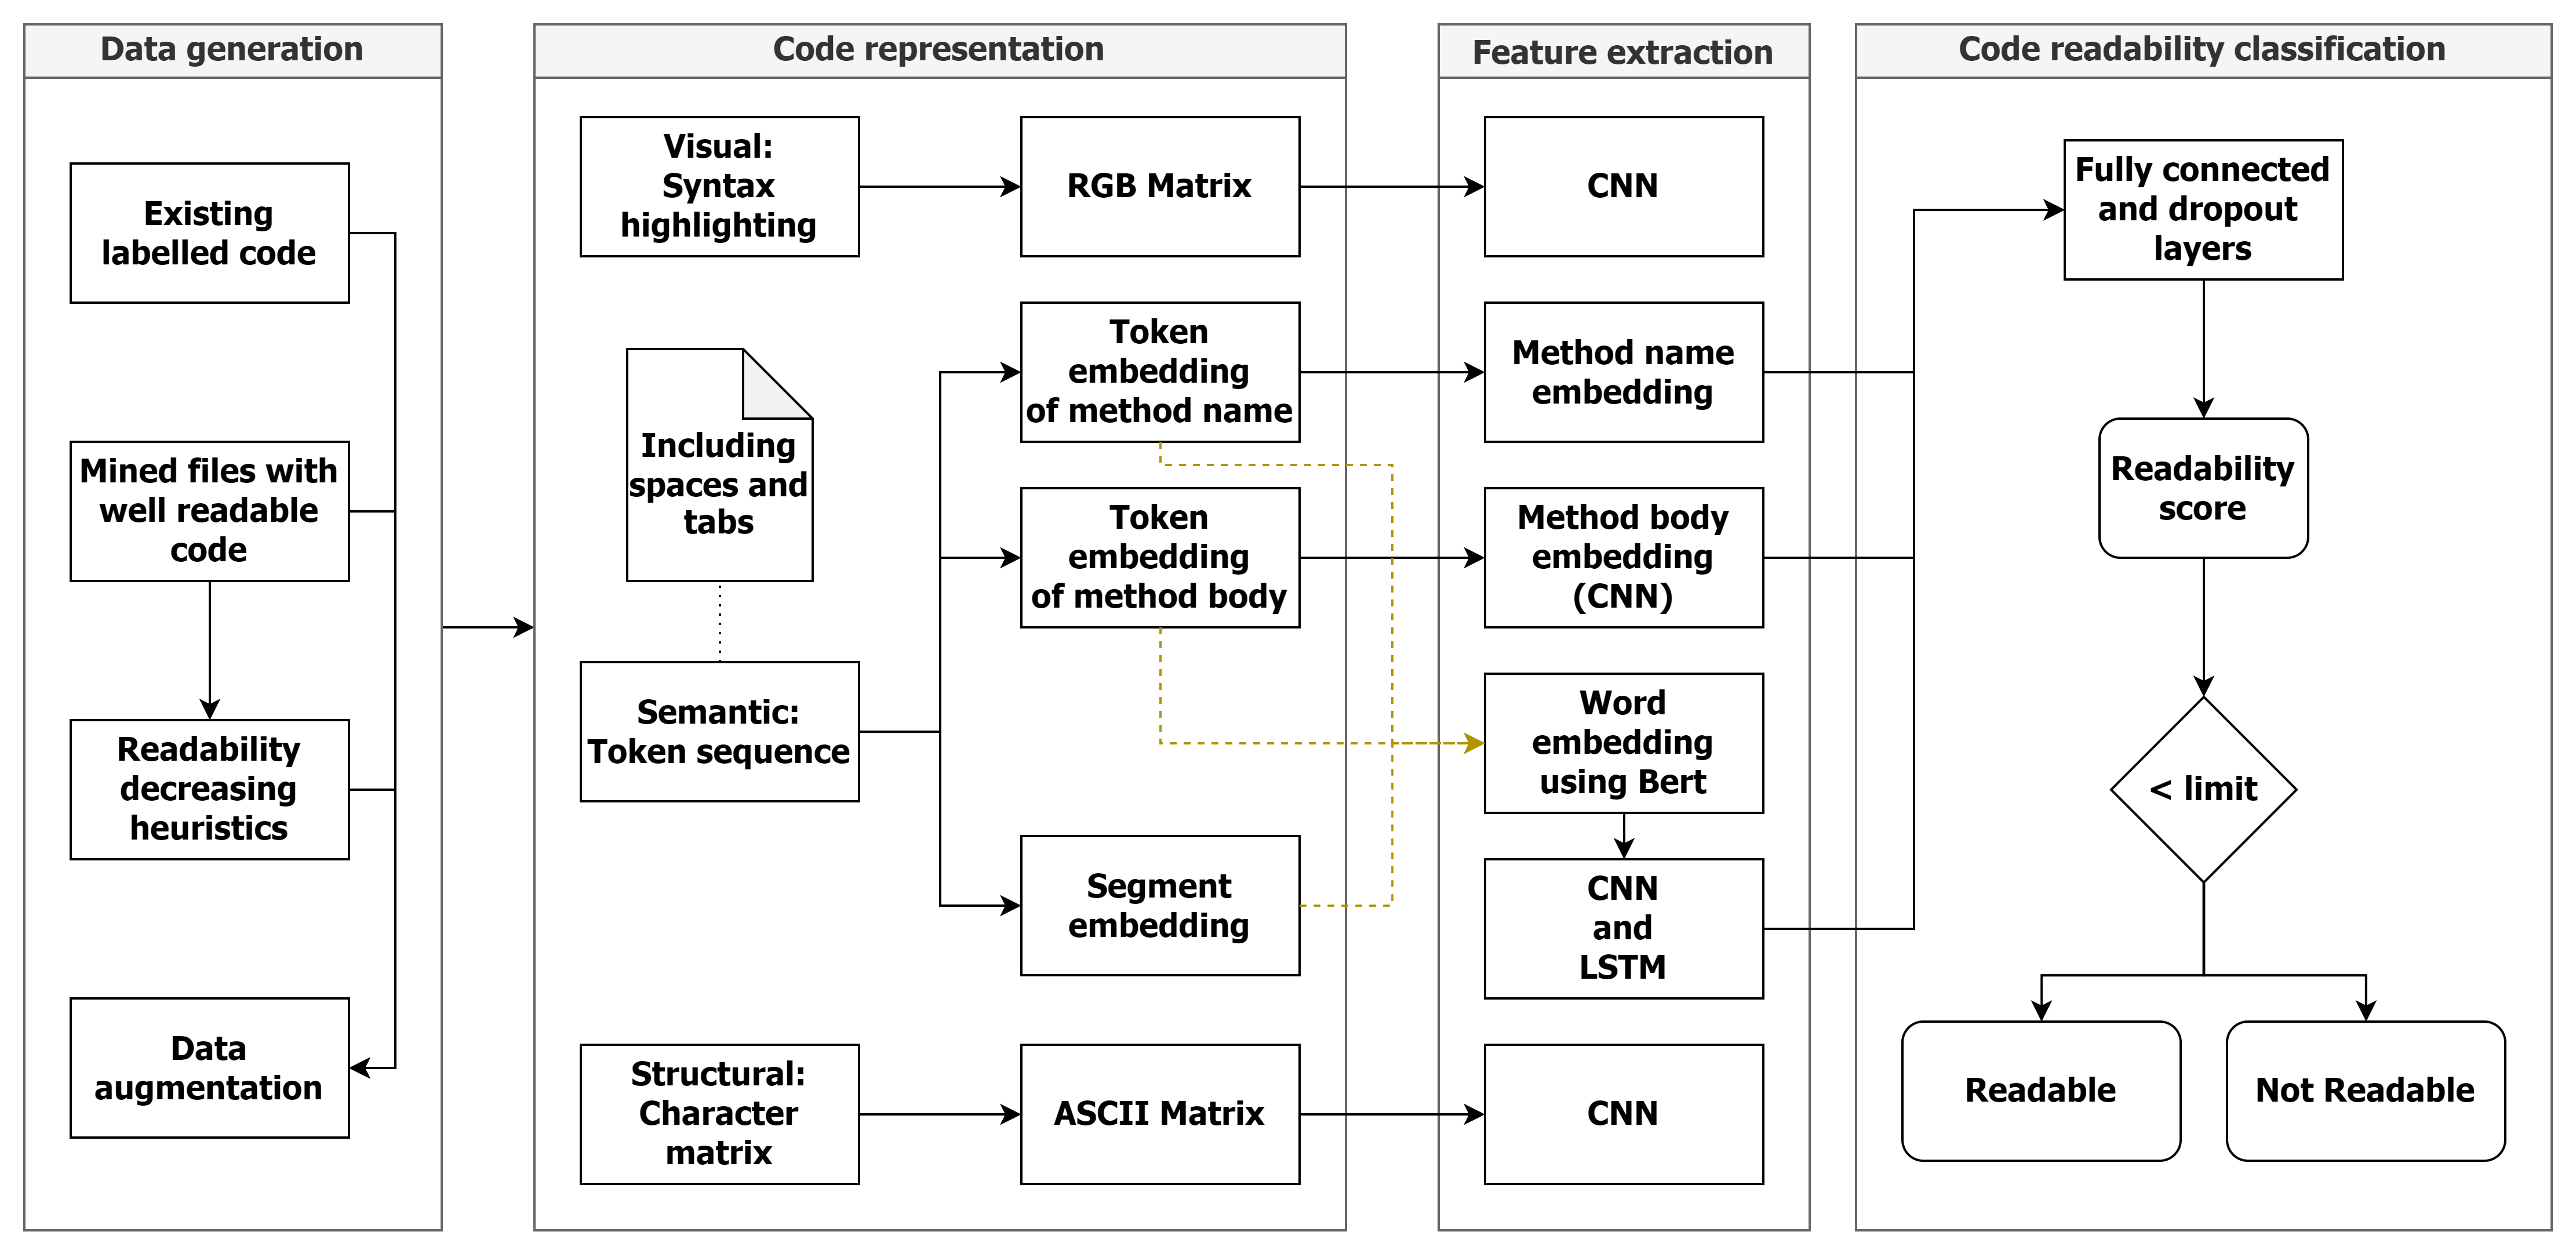
\includegraphics[width=\textwidth]{Model_pipeline.png}
		\caption{Overview of the planned approach.}
		\label{fig:model_pipeline}
	\end{figure}
	
	% TODO: Inline this in research questions?
	% \subsection{Data generation} \label{Data generation}
	Deep Learning based models perform better the more training data they get~\cite{hestness2017deep}. Therefore, one approach in order to further improve existing models is to gather more training data.
	This requires, as it was done previously, a lot of effort and persons willing to rate code based on their readability. We present another approach for gathering training data.
	
	In a first step, GitHub repositories with known high code quality are downloaded and labeled as highly readable. We select repositories using a similar approach as \citeauthor{allamanis2016convolutional}~\cite{allamanis2016convolutional} and then assume that they contain only well readable code.
	In a second step, the code is manipulated so that it is subsequently less readable. This approach is similar to the approach of \citeauthor{loriot2022styler}~\cite{loriot2022styler}. After both steps, we have a new, automatically generated training dataset for source code readability classification.
		
	% Readabililty Decreasing Heuristics
	This brings up the question, how to manipulate code so that it is less readable afterwards. We therefore introduce a tool called Readability Decreasing Heuristics. As the name suggests this is a collection of heuristics that, when applied to source code, lower the readability of it. For example such a heuristic is to replace spaces with newlines. Another example is to increase the indentation of a code block by a tab or multiple spaces. Moreover, with most changes it is also possible to do exactly the opposite (replacing newlines with spaces, decreasing indentation), which in most cases also decreases the readability of source code.
	
	Code snippets in Java are syntactically the same, before and after applying Readability Decreasing Heuristics. Complexity did not change either. However, if various modifications are applied many times, those changes are capable of lowering the readability of source code, as the comparison of listing~\ref{lst:cassandra-src-java-org-apache-cassandra-utils} and listing~\ref{lst:cassandra-src-java-org-apache-cassandra-utils-modified} suggests.
	
	Note that we assume two things for the data generation approach:
	\begin{enumerate}[label={Assumption \arabic*},ref={\arabic*},leftmargin=*]
		\item \label{well-readable-assumption} \textbf{(well-readable-assumption)} The selected repositories contain only well-readable code.
		\item \label{poorly-readable-assumption} \textbf{(poorly-readable-assumption)} After applying Readability Decreasing Heuristics, the code is poorly readable.
	\end{enumerate}
	
	% Model modifications/Further improvements
	\label{model-modifications}
	In recent years it was shown that Deep Learning models can be further improved by modifying the structure of the architecture or by introducing new components, parts or layers to existing architectures. 
	We suggest two improvements for the model of \citeauthor{mi2022towards}~\cite{mi2022towards}. Firstly, we want to embed spaces and tabs as semantic tokens. Secondly, adding a method name fitting classifier as a component of the overall model could be an improvement.
	% Surpassing
	\label{suggestions}If there is time left, we will try to surpass the performance of recent source code readability classifiers with those improvements to data generation and the model.
	%, such as the model proposed by \citeauthor{mi2022towards}~\cite{mi2022towards}.
	
	% We suggest two improvements for the model of \citeauthor{mi2022towards}~\cite{mi2022towards}:
	%\begin{enumerate}
	%	\item \label{embedding-spaces-component} \textbf{(embedding-spaces-component)} Embedding spaces and tabs as semantic tokens.
	%	\item \label{name-classifier-component} \textbf{(name-classifier-component)} Adding a method name fitting classifier as a component of % the overall model.
	%\end{enumerate}
	
	We will evaluate our suggestions with two methods. Firstly, we conclude a user study. Secondly, we compare code readability models with each other.
	
	\pagebreak
	
	\subsection{User study}\label{user-study}
	% We will conclude a user study to evaluate the newly generated data for readability classifier models.
	The goal of the user study is to answer the following key questions:
	
	\begin{enumerate}
		\item Does the well-readable-assumption (assumption \ref{well-readable-assumption}) hold?
		\item Does the poorly-readable-assumption (assumption \ref{poorly-readable-assumption}) hold?
	\end{enumerate}
	
	We will achieve this by showing programmers code snippets that were generated with the presented approach. Therefore, human annotators give each code snippet a rating of its readability. The annotators are selected by prolific\curl{https://www.prolific.com/}{2023-09-30}. Particular attention is paid to a high proportion of people from industry. The readability rating is based on a five-point Likert scale~\cite{likert1932technique} ranging from one (i.e., very unreadable) to five (i.e., very readable). We apply the same rating as done previously~\cite{buse2009learning, dorn2012general, scalabrino2016improving}, but, other than before, we will not use the rating for labeling the training data. Instead, we will only use the ratings to validate a few randomly selected code snippets out of many that are automatically labeled.
		
	\subsection{Comparing models}\label{compare-models}
	Besides the user study we will evaluate our suggestions by comparing machine learning models against each other.
	The comparisons are based on common metrics such as accuracy, F1-score and MCC~\cite{chicco2020advantages}. One can distinguish further between the following variants of comparing models:
	
	In one variant we compare models that have the same architecture (same layers, same weight initialization, same components, etc.) while they differ in the data they are trained on. For example, we can train a model with the old and new datasets, separately and combined. If done for multiple model architectures we can evaluate how the differences in training data influence the model performance. 
	
	Another variant would be to compare models with different architecture but the same training data. In this way, we can evaluate newly introduced components by measuring and comparing the performance of such models.

	A third comparison variant is created by combining the first two. Both of them lead to many options in what to compare, especially if only small changes to training data or model architecture are done. To find out, if our suggestions lead to a better model overall, we will compare our newly created model with all changes at once to the state-of-the-art model of \citeauthor{mi2022towards}~\cite{mi2022towards}.
	
	\subsection{Research questions}\label{research-questions}
	We come up with the following research questions:
	
%	\begin{resq}What is the quality of our new approach for data generation?\end{resq} \label{RQ1}
%	Until now, the data for readability classification was generated manually. Therefore, human annotators ranked code snippets by their readability level based on a five-point Likert scale~\cite{likert1932technique} ranging from one (i.e., very unreadable) to five (i.e., very readable)~\cite{buse2009learning, dorn2012general, scalabrino2016improving}. Our new data will be generated in an automatic approach, where no manual labeling of code is necessary. We want to compare the quality of this data to the data used for previous models.
	
	\begin{resq} \textbf{(select-well)} Can automatically selected code be assumed to be well readable?\end{resq} \label{select-well}
	In our new approach for generating training data, we assume that the code from repositories is readable under certain conditions (assumption~\ref{well-readable-assumption}). We want to check whether that holds. To answer this question we will use the results of the user study (section~\ref{user-study}).
	
	\begin{resq} \textbf{(generate-poor)} Can poorly readable code be generated from well readable code?\end{resq} \label{generate-poor}
	It is not sufficient to have only well readable code for training a classifier. We also need poorly readable code. Therefore, we will try to generate such code from the well readable code. We will investigate whether this is possible in principle, and we will propose an automated approach for archiving this: Readability Decreasing Heuristics.
	
	As the name already suggests, the applied transformations on the source code are only heuristics. To answer, whether the generated code is badly readable (assumption~\ref{poorly-readable-assumption}) we will utilize the results of the user study (section~\ref{user-study}).
	
	\begin{resq} \textbf{(best-heuristics)} Which heuristics are best to generate poorly readable code from well readable code?\end{resq} \label{best-heuristic}
	We want to compare the modifications of the proposed heuristics for generating poorly readable code to each other. Therefore we will train the same classifier model with badly readable code generated by different Readability Decreasing Heuristics. We will then evaluate the model variations against each other (section~\ref{compare-models}) to answer the research question.
	
	\begin{resq} \textbf{(new-data)} To what extent can the new data improve existing readability models?\end{resq} \label{new-data}
	It was shown that Deep Learning models get better the more training data is available~\cite{hestness2017deep}. This holds under the assumption that the quality of the data is the same or at least similar. We want to check if the quality of our new data is sufficient for improving the Deep Learning based readability classifier of \citeauthor{mi2022towards}~\cite{mi2022towards}. Therefore we will train their proposed model with and without the new data and then evaluate the models against each other (section~\ref{compare-models}).
	
	% Next RQ on new page
	\pagebreak
	
%	\begin{resq} \textbf{(model-modifications)} Optional: How can existing Deep Learning approaches be further improved?\end{resq} \label{model-modifications}
%	In recent years it was shown that Deep Learning models can be further improved by modifying the structure of the architecture or by introducing new components, parts or layers to existing architectures. We suggest two improvements for the model of \citeauthor{mi2022towards}~\cite{mi2022towards}: Embedding spaces and tabs as semantic tokens and adding a method name fitting component. We will evaluate the proposed improvements as described earlier~\ref{suggestions}.
	
	\begin{resq} \textbf{(embedding-spaces)} Optional: To what extend does the embedding of spaces and tabs in semantic code representations improve readability classification?\end{resq} \label{embedding-spaces}
	The state-of-the-art model of \citeauthor{mi2022towards}~\cite{mi2022towards} does consider spaces and tabs only in its visual component. We want to investigate if it can improve the quality of a Deep Learning based model if spaces and tabs are encoded as semantic tokens. We also want to investigate if this makes the visual component superfluous. We will evaluate the proposed improvement as described earlier (section~\ref{compare-models}).
	
	\begin{resq} \textbf{(name-classifier)} Optional: To what extend does the usage of a method name classifier improve readability classification?\end{resq} \label{name-classifier}
	Correct naming of identifiers is crucial for ensuring readability of software programs. It is of outstanding importance for readability of code that the name of methods fit the method bodies~\cite{liu2019learning}. We want to introduce a new component to the model of \citeauthor{mi2022towards}~\cite{mi2022towards} that is built similar to Code2Vec~\cite{alon2019code2vec}. We want to investigate if the newly introduced component improves the quality of the resulting model. We will evaluate the proposed improvement as previously described (section~\ref{compare-models}).
	
	\backmatter
	
	\printbibliography
	
\end{document}
